%!TEX TS-program = LuaLaTeX
\documentclass[tikz,border=0.5cm]{standalone}
\usetikzlibrary{shapes}
\pdfvariable suppressoptionalinfo \numexpr32+64+512\relax

\begin{document}
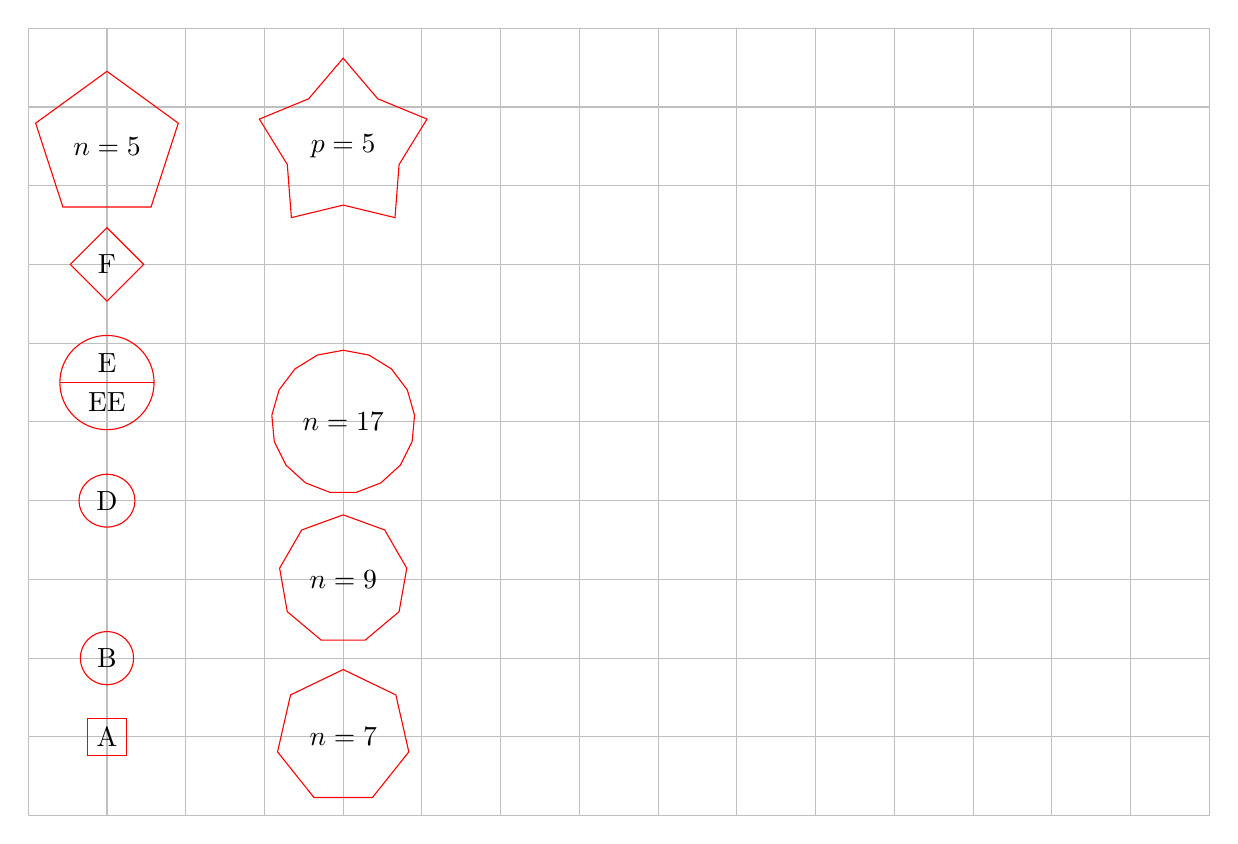
\begin{tikzpicture}
\draw[step=1cm,lightgray,thin] (0,0) grid (15,10);
\node[rectangle,draw=red] (a) at (1,1){A};
\node[circle,draw=red] (b) at (1,2){B};
\node[coordinate,draw=red] (c) at (1,3){C};

\node[ellipse,draw=red] (d) at (1,4){D};
\node[circle split,draw=red] (e) at (1,5.5){E \nodepart{lower}EE};

\node[diamond,draw=red] (f) at (1,7){F};

\node[draw=red,regular polygon,regular polygon sides=5] at (1,8.5) {$n=5$};
\node[draw=red,regular polygon,regular polygon sides=7] at (4,1) {$n=7$};
\node[draw=red,regular polygon,regular polygon sides=9] at (4,3) {$n=9$};
\node[draw=red,regular polygon,regular polygon sides=17] at (4,5) {$n=17$};

 \node[draw=red,star,star points=5] at (4,8.5) {$p=5$};
\end{tikzpicture}
\end{document}
 
 
% rectangle, circle, and coordinate are always defined
% rest via shapes library